\documentclass[a4paper, 11pt]{exam}
\usepackage[T1]{fontenc}
\usepackage{titling}
\usepackage{url}
\usepackage{amsmath,amsthm,amssymb}
\usepackage{graphicx}
\usepackage{graphics}
\usepackage{listings}
\usepackage[dvipsnames]{xcolor}
\usepackage{tabularx}
\usepackage{ragged2e}
\usepackage{courier}
\usepackage{textcomp}
\usepackage{circuitikz}
\usepackage{tikz}
\usepackage{enumitem}
\usepackage{karnaugh-map}
\usepackage{bytefield}
\usepackage{mathrsfs}
\usepackage{cancel}
\usepackage[linesnumbered,ruled,vlined]{algorithm2e}
\usepackage{hyperref}
\newcommand{\invlaplace}[1]{%
\mathscr{L}^{-1}\left\{#1\right\}
}
\usepackage{tikz}
\usetikzlibrary{patterns}
\newcommand{\plotROC}[3]{
    % Draw the axes
    \draw[->] (-2.5,0) -- (2.5,0) node[anchor=north, xshift=.5cm, yshift=.3cm] {\( \text{Re}(z) \)};
    \draw[->] (0,-2.5) -- (0,2.5) node[anchor=east , xshift=.5cm, yshift=.2cm] {\( \text{Im}(z) \)};
    
    % Draw the Legend
    \draw (2.5,2.5) rectangle (4,1.5);
    \fill[red] (2.8,1.7) circle [radius=.05];
    \node[anchor=west] at (2.9, 1.7) {Poles};
    \fill[black] (2.8,2.2) circle [radius=.05];
    \node[anchor=west] at (2.9, 2.2) {Zeros};

    % Draw the circle with radius passed in
    \draw[dashed] (0,0) circle [radius=#1];

    % Plot poles
    \foreach \x/\y in {#2} {
      \fill[black] (\x,\y) circle [radius=.05];
    }

    % Plot zeros
    \foreach \x/\y in {#3} {
      \fill[red] (\x,\y) circle [radius=.05];
    }

    % Label the ROC
    \node at (1.5,1.5) {ROC};

    % Draw the circle to indicate it's not part of the ROC
    \draw[dashed] (0,0) circle [radius=#1];
}


\newcommand{\cc}[2]{
  \textcolor{red}{\cancelto{\textcolor{black}{#2}}{\textcolor{black}{#1}}}
}

\newcommand{\laplace}[1]{%
\mathscr{L}\left\{#1\right\}
}
\newcommand{\fourier}[1]{%
\mathscr{F}\left\{#1\right\}
}

\newcommand{\ztransform}[1]{%
\mathscr{Z}\left\{#1\right\}
}

\newcommand{\wfbrac}[1]{%
\left[ \,#1\right] \,
}
\newcommand{\wfcbrac}[1]{%
\left\{ \,#1\right\} \,
}
\newcommand{\wfparen}[1]{%
\left(#1\right)
}

\newcommand{\subtitle}[1]{%
  \posttitle{%
    \par\end{center}
    \begin{center}\large#1\end{center}
    }%
}

\usepackage{environ}

\NewEnviron{eqnsection}[2]{%
  \newcommand{\myvspace}{#1}%
  \vspace{\myvspace}%
  \begin{align*}
  \intertext{#2}
  \BODY
  \end{align*}%
  \vspace{\myvspace}%
}


\newcommand{\uparrowat}[1]{\underset{\uparrow}{#1}}


\newlist{myenumerate}{enumerate}{2}
\setlist[myenumerate,1]{label=\roman*)}
\setlist[myenumerate,2]{label=\alph*)}



\newcommand\tab[1][1cm]{\hspace*{#1}}

\renewcommand{\labelenumi}{\alph{enumi})}

\title{Homework Assignment \#3}
\subtitle{ECE 6530: Digital Signal Processing \\
\today\\}
\author{ Miguel Gomez U1318856\\
\textbf{Homework set \#3}}
\date{Due Date: Sep 29, 2023\\
(75 points)}

\begin{document}
\maketitle
\section{Problem 3.2 parts a, b, d, f, and h}
Determine the z-transform of the following signals and sketch the ROC of the following \textcolor{Red}{Note*} I didn't catch it before, but the enumeration below is off. The letters above are the correct ones.
\begin{enumerate}
\item $x(n) = (1+n)u(n)$
\item $x(n) = (a^{n} + a^{-n})u(n)$ real $a$
\item $x(n) = (na^{n}\sin{\omega_0n})u(n)$
\item $x(n) = Ar^n\cos{\wfparen{\omega_0n + \phi}}u(n)$
\item $x(n) = \wfbrac{\frac{1}{2}}^{n}[u(n)-u(n-10)]$
\end{enumerate}
\begin{eqnsection}{0em}{a) Problem a can be split into two parts:}
  x(n) &= (1+n)u(n) = u(n) + nu(n)
  \intertext{The first is a simple one that we can solve by geometric sum. But we have a table in the book that has these simple cases so we can skip ahead a bit:}
  X_{tot}(z) &= X_1(z) + X_2(z) \\
  X_{tot}(z) &= \wfbrac{\frac{1}{1-z^{-1}}} - z\frac{dX(z)}{dz} \\
  X_{tot}(z)&= \wfbrac{\frac{1}{1-z^{-1}}} - z\wfbrac{\frac{-1}{(1-z^{-1})^2}}(z^{-2}) \\
  X_{tot}(z)&= \wfbrac{\frac{1}{1-z^{-1}}} + \wfbrac{\frac{z^{-1}}{(1-z^{-1})^2}} \\
  X_{tot}(z)&= \wfbrac{\frac{1-z^{-1}}{(1-z^{-1})^2}} + \wfbrac{\frac{z^{-1}}{(1-z^{-1})^2}} \\
  X_{tot}(z)&=\wfbrac{\frac{1}{(1-z^{-1})^2}} \\
  \intertext{The poles are clearly at 1 since a value of 1 for $z$ would cause the denominator to go to 0. The zeros would need us to multiply top and bottom by $z^{2}$.}
  X_{tot}(z)&=\wfbrac{\frac{z^2}{z^2(1-z^{-1})^2}}=\wfbrac{\frac{z^2}{(z-1)^2}} \\
  \intertext{This shows the zeros as well as the poles. both with multiplicity 2.}
\end{eqnsection}
\begin{center}
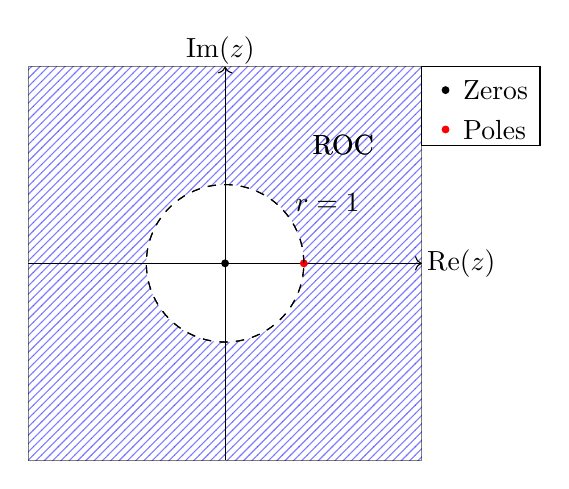
\begin{tikzpicture}
  % Fill the region outside the circle
  \filldraw[pattern=north east lines, pattern color=blue, opacity=0.5] (-2.5,-2.5) rectangle (2.5,2.5);
  \fill[white] (0,0) circle [radius=1];
  \plotROC{1}{0/0}{1/0}
  % Label the ROC
  \node at (1.5,1.5) {ROC};
  \node[anchor=west] at (1/1.3, 1/1.3) {\( r = 1 \)};
\end{tikzpicture}
\end{center}
\begin{eqnsection}{0em}{b) }
  x(n) &= (a^{n} + a^{-n})u(n) =  a^{n}u(n) + a^{-n}u(n) \\
  &= \sum_{n=-\infty}^{\infty}a^{n}u(n) + \sum_{n=-\infty}^{\infty}a^{-n}u(n)
  \intertext{using the definition of the transform, we can now introduce $z^{-1}$ and absorb the $u(n)$ into the sum:}
  &= \sum_{n=0}^{\infty}a^{n}z^{-1} + \sum_{n=0}^{\infty}a^{-n}z^{-1} \\
 X_1(z) &= \frac{1}{1-az^{-1}} \\
 X_2(z) &= \frac{1}{1-(az)^{-1}} \\
 \intertext{combining the two into a single fraction:}
 &= \frac{1}{1-az^{-1}} + \frac{1}{1-(az)^{-1}} = \frac{1-(az)^{-1}}{(1-(az)^{-1})(1-az^{-1})} + \frac{1-az^{-1}}{(1-(az)^{-1})(1-az^{-1})}\\
 &=\frac{1-az^{-1} + 1 - (az)^{-1}}{(1-(az)^{-1})(1-az^{-1})} = \frac{2 - az^{-1} - (az)^{-1}}{(1-(az)^{-1})(1-az^{-1})}\\
\end{eqnsection}
\newpage
\begin{eqnsection}{0em}{the zeros and the poles can be found by evaluating the top and bottom of the expression as we did in a) and we start with the poles:}
  (1-(az)^{-1})(1-az^{-1})&= 0 \\
  X_{poles} &= \wfcbrac{a,a^{-1}}\\
  \textcolor{red}{z}(2 - az^{-1} - a^{-1}z^{-1}) &= 0\textcolor{red}{z}\\
  2z - (a + a^{-1}) &= 0\\
  X_{zero} &= \wfcbrac{\frac{a + a^{-1}}{2}} 
\end{eqnsection}
\begin{center}
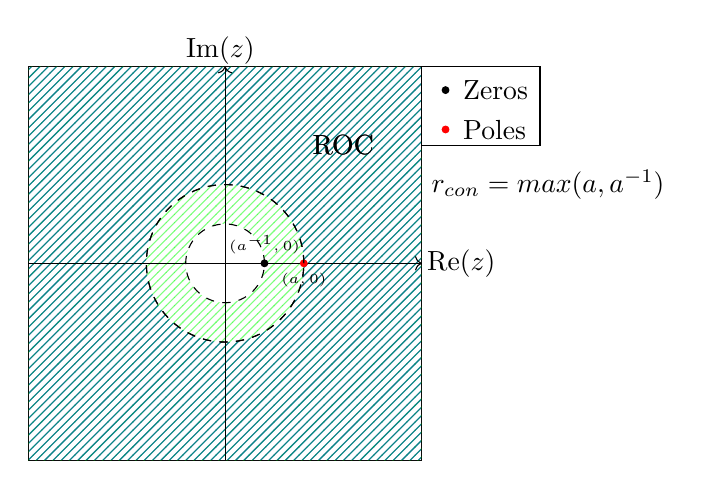
\begin{tikzpicture}
  % Fill the region outside the circle
  \filldraw[pattern=north east lines, pattern color=blue, opacity=0.9] (-2.5,-2.5) rectangle (2.5,2.5); 
  \fill[white] (0,0) circle [radius=1];
  \filldraw[pattern=north east lines, pattern color=green, opacity=0.5] (-2.5,-2.5) rectangle (2.5,2.5);
  \fill[white] (0,0) circle [radius=.5];
  \draw[dashed] (0,0) circle [radius=.5];
  \plotROC{1}{0.5/0}{1/0}
  % Label the ROC
  \node at (1.5,1.5) {ROC};
  \node[anchor=west] at (2.5, 1) {\( r_{con} = max(a,a^{-1}) \)};
  \node[anchor=north,font=\tiny] at (1,0) {\((a,0)\)};
  \node[anchor=south,font=\tiny] at (.5,0) {\((a^{-1},0)\)};
\end{tikzpicture}
\end{center}
ROC here is whichever of the two, $a$ or $a^{-1}$ is larger.
\begin{eqnsection}{0em}{c)}
  x(n) &= (na^{n}\sin{\wfparen{\omega_0n})}u(n)\\
  \intertext{The inclusion of the $n$ in the expression means we need to do the derivative, and we can take the rest together as a whole:}
  &= n(a^{n}\sin{\wfparen{\omega_0n}})u(n)\\
  nx(n) &= -z\frac{dX(z)}{dz}\\
  &= -z\wfparen{\frac{d}{dz}\cdot\frac{az^{-1}\sin{\wfparen{\omega_0}}}{1-2az^{-1}\cos{\wfparen{\omega_0} + a^{2}z^{-2}}}}\\
  \text{by  }\frac{d}{dz}\frac{f(z)}{g(z)}&= \frac{f'g - fg'}{g^2}\\
  = -z\wfparen{\frac{(-1)az^{-2}\sin{\wfparen{\omega_0}}\cdot(1-2az^{-1}\cos{\wfparen{\omega_0} + a^{2}z^{-2}})}{\wfparen{1-2az^{-1}\cos{\wfparen{\omega_0} + a^{2}z^{-2}}}^{2}}} &+\\
  -z\wfparen{\frac{az^{-1}\sin{\wfparen{\omega_0}}\cdot((-1)(-2)az^{-2}\cos{\wfparen{\omega_0} + (-2)a^{2}z^{-3}})} {\wfparen{1-2az^{-1}\cos{\wfparen{\omega_0} + a^{2}z^{-2}}}^{2}}}\\
\end{eqnsection}
\begin{eqnsection}{-3em}{}
   X(z) = 
  -z\wfparen{\frac{-az^{-2}\sin{\wfparen{\omega_0}}\cdot(1-2az^{-1}\cos{\wfparen{\omega_0} + a^{2}z^{-2}})}{\wfparen{1-2az^{-1}\cos{\wfparen{\omega_0} + a^{2}z^{-2}}}^{2}}} +\\
  -z\wfparen{\frac{az^{-1}\sin{\wfparen{\omega_0}}\cdot(2az^{-2}\cos{\wfparen{\omega_0} - 2a^{2}z^{-3}})} {\wfparen{1-2az^{-1}\cos{\wfparen{\omega_0} + a^{2}z^{-2}}}^{2}}}\\
\end{eqnsection}
\begin{eqnsection}{0em}{Combining into a single fraction:}
  &=  -z\wfparen{\frac{-az^{-2}\sin{\wfparen{\omega_0}}\cdot(1-2az^{-1}\cos{\wfparen{\omega_0} - a^{2}z^{-2}}) + az^{-1}\sin{\wfparen{\omega_0}}\cdot(2az^{-2}\cos{\wfparen{\omega_0} + 2a^{2}z^{-3}})} {\wfparen{1-2az^{-1}\cos{\wfparen{\omega_0} + a^{2}z^{-2}}}^{2}}}\\
  &= -zaz^{-1}\sin{\wfparen{\omega_0}}\cdot\wfparen{\frac{z^{-1}(1-2az^{-1}\cos{\wfparen{\omega_0} + a^{2}z^{-2}}) + (2az^{-2}\cos{\wfparen{\omega_0} - 2a^{2}z^{-3}})} {\wfparen{1-2az^{-1}\cos{\wfparen{\omega_0} + a^{2}z^{-2}}}^{2}}}\\
  &= -a\cc{zz^{-1}}{1}\sin{\wfparen{\omega_0}}\cdot\wfparen{\frac{(z^{-1}-2az^{-2}\cos{\wfparen{\omega_0} + a^{2}z^{-3}}) + (2az^{-2}\cos{\wfparen{\omega_0} - 2a^{2}z^{-3}})} {\wfparen{1-2az^{-1}\cos{\wfparen{\omega_0} + a^{2}z^{-2}}}^{2}}}\\
  &= -a\sin{\wfparen{\omega_0}}\cdot\wfparen{\frac{z^{-1}-2az^{-2}\cos{\wfparen{\omega_0}} + a^{2}z^{-3} + 2az^{-2}\cos{\wfparen{\omega_0} - 2a^{2}z^{-3}}} {\wfparen{1-2az^{-1}\cos{\wfparen{\omega_0} + a^{2}z^{-2}}}^{2}}}\\
  &= -a\sin{\wfparen{\omega_0}}\cdot\wfparen{\frac{z^{-1}+\cc{(2a - 2a)}{0}z^{-2}\cos{\wfparen{\omega_0} + \cc{(2a^{2} - 2a^{2})}{0}z^{-3}}} {\wfparen{1-2az^{-1}\cos{\wfparen{\omega_0} + a^{2}z^{-2}}}^{2}}}\\
  &= \frac{-az^{-1}\sin{\wfparen{\omega_0}}}{\wfparen{1-2az^{-1}\cos{\wfparen{\omega_0} + a^{2}z^{-2}}}^{2}}
  \intertext{Unfortunately, I believe I dropped a negative somewhere and I am not able to see where. It should have two terms because the exponential form has two terms. Doing it using the exponential instead. We could use these, but I am calling it here and stating the results we obtained in our study session group together: }
  &= \frac{\wfparen{az^{-1} - a^{-3}z^{-3}}\sin{\wfparen{\omega_0}}}{\wfparen{1-2az^{-1}\cos{\wfparen{\omega_0}} + a^{2}z^{-2}}^{2}}
\end{eqnsection}
\begin{center}
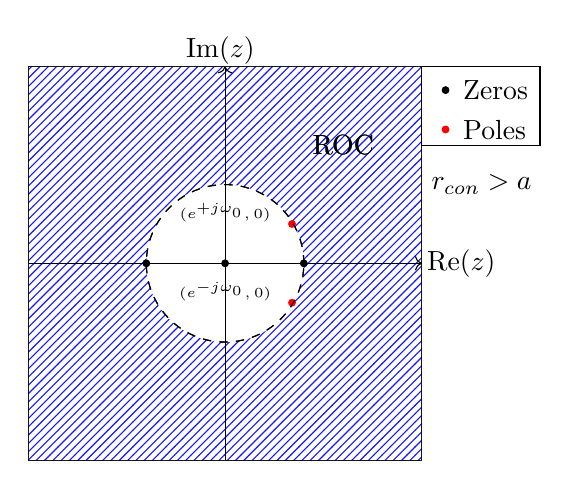
\begin{tikzpicture}
  % Fill the region outside the circle
  \filldraw[pattern=north east lines, pattern color=blue, opacity=0.9] (-2.5,-2.5) rectangle (2.5,2.5); 
  \fill[white] (0,0) circle [radius=1];
  \plotROC{1}{0/0,1/0,-1/0}{.85/.5,.85/-.5}
  % Label the ROC
  \node at (1.5,1.5) {ROC};
  \node[anchor=west] at (2.5, 1) {\( r_{con} > a \)};
  \node[anchor=south,font=\tiny] at (0,.4) {\((e^{+j\omega_0},0)\)};
  \node[anchor=south,font=\tiny] at (0,-.6) {\((e^{-j\omega_0},0)\)};
\end{tikzpicture}
\end{center}
ROC here is greater than $a$, double poles at $e^{\pm j\omega_0}$, zeros at $\pm a$ and $0$. The choice to place poles where they are in the plot is arbitrary.

\begin{eqnsection}{-2em}{d)}
  x(n) &= Ar^n\cos{\wfparen{\omega_0n + \phi}}u(n)
  \intertext{Note, we can use the definition of cos as the exponential to extract the phase term from the expression.}
  \cos(\theta) &= \frac{e^{i\theta} + e^{-i\theta}}{2}\\
  \cos{\wfparen{\omega_0n + \phi}} &= \frac{e^{i\omega_0n  + \phi} + e^{-i\omega_0n  - \phi}}{2}\\
   &= \frac{e^{i\omega_0n}e^{i\phi} + e^{-i\omega_0n}e^{-i\phi}}{2}\\
  x(n) &= Ar^n\wfparen{\frac{e^{i\omega_0n}e^{i\phi} + e^{-i\omega_0n}e^{-i\phi}}{2}}u(n)\\
  x(n) &= Ar^n\wfparen{\frac{e^{i\omega_0n}e^{i\phi}}{2} + \frac{e^{-i\omega_0n}e^{-i\phi}}{2}}u(n)\\
  X(z) &= \frac{A}{2}\wfbrac{\frac{e^{i\phi}}{1-re^{i\omega_0}z^{-1}} + \frac{e^{-i\phi}}{1-re^{-i\omega_0}z^{-1}}}\\
  \intertext{Combining the fractions:}
  &= \frac{A}{2}\wfbrac{\frac{e^{i\phi}(1-re^{-i\omega_0}z^{-1})}{(1-re^{-i\omega_0}z^{-1})(1-re^{i\omega_0}z^{-1})} + \frac{e^{-i\phi}(1-re^{i\omega_0}z^{-1})}{(1-re^{i\omega_0}z^{-1})(1-re^{-i\omega_0}z^{-1})}}\\
  &=\frac{A}{2}\wfbrac{\frac{e^{i\phi}+e^{-i\phi}-rz^{-1}(e^{i\omega_0}e^{-i\phi}+e^{-i\omega_0}e^{i\phi})}{(1-r(e^{i\omega_0} + e^{-i\omega_0})+r^{2}z^{-2})}}\\
  &=\frac{A}{2}\wfbrac{\frac{e^{i\phi}+e^{-i\phi}-rz^{-1}(e^{i\omega_0}e^{-i\phi}+e^{-i\omega_0}e^{i\phi})}{(1-rz^{-1}(e^{i\omega_0} + e^{-i\omega_0})+r^{2}z^{-2})}}\\
  \intertext{Note: we can distribute the $\frac{1}{2}$ into the top and apply it to the expontentials. additionally, we can modify the bottom by multiplying the middle factor by $\frac{2}{2}$}
  &=A\wfbrac{\frac{\frac{e^{i\phi}+e^{-i\phi}}{2}-rz^{-1}\frac{(e^{i\omega_0-i\phi}+e^{-i\omega_0+i\phi})}{2}}{(1-r2z^{-1}\frac{e^{i\omega_0} + e^{-i\omega_0}}{2}+r^{2}z^{-2})}}\\
\therefore  X(z) &=A\wfbrac{\frac{\cos{(\phi)}-rz^{-1}\cos{(\omega_0-\phi)}}{(1-r2z^{-1}\cos{(\omega_0)}+r^{2}z^{-2})}}\\\\
\intertext{Poles at $z = re^{j\omega_0}$ and $z = ae^{-j\omega_0}$ and zeros at $z = 0$, and $z = r\frac{\cos{(\omega_0 - \phi)}}{\cos{(\phi)}}$.
Triple pole at $z = \frac{1}{3}$ and zeros at $z = 0$ and $z = \frac{1}{3}$, so there is a pole-zero cancellation.}
\end{eqnsection}
\newpage
\begin{center}
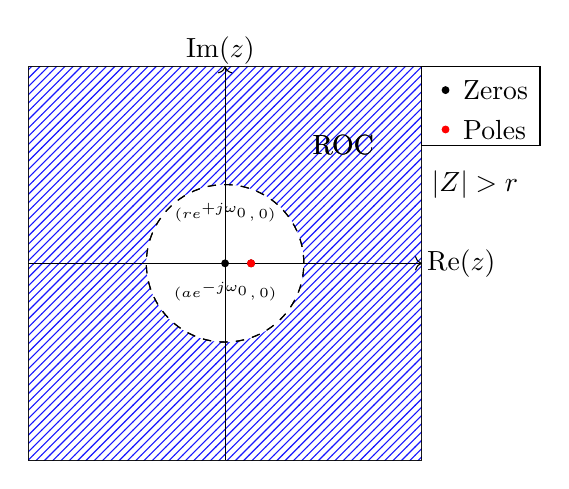
\begin{tikzpicture}
  % Fill the region outside the circle
  \filldraw[pattern=north east lines, pattern color=blue, opacity=0.9] (-2.5,-2.5) rectangle (2.5,2.5); 
  \fill[white] (0,0) circle [radius=1];
  \plotROC{1}{.33/0,0/0}{.33/0,.33/0}
  % Label the ROC
  \node at (1.5,1.5) {ROC};
  \node[anchor=west] at (2.5, 1) {\( |Z| > r \)};
  \node[anchor=south,font=\tiny] at (0,.4) {\((re^{+j\omega_0},0)\)};
  \node[anchor=south,font=\tiny] at (0,-.6) {\((ae^{-j\omega_0},0)\)};
\end{tikzpicture}
\end{center}
\begin{eqnsection}{-2em}{h)}
  x(n) &= \wfparen{\frac{1}{2}}^{n}[u(n)-u(n-10)] = \wfparen{\frac{1}{2}}^{n}u(n)-\wfparen{\frac{1}{2}}^{10}\wfparen{\frac{1}{2}}^{n-10}u(n-10)\\
  x(n) &= \frac{1}{1-\frac{1}{2}z^{-1}}-\frac{\wfparen{\frac{1}{2}}^{10}z^{-10}}{1-\frac{1}{2}z^{-1}}\\
  x(n) &= \frac{1-\wfparen{\frac{1}{2}}^{10}z^{-10}}{(1-\frac{1}{2}z^{-1})^{2}}\\
  \intertext{Here, we can see that we will have zeros at $z = \frac{1}{2}e^{\frac{j2\pi n}{M}}$ with multiplicity 10, and poles at $z = \frac{1}{2}$ with multiplicity 2.}
\end{eqnsection}
\begin{center}
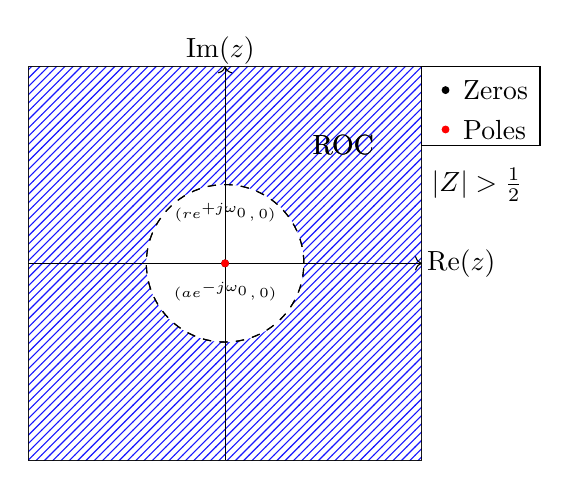
\begin{tikzpicture}
  % Fill the region outside the circle
  \filldraw[pattern=north east lines, pattern color=blue, opacity=0.9] (-2.5,-2.5) rectangle (2.5,2.5); 
  \fill[white] (0,0) circle [radius=1];
  \plotROC{1}{0/0}{0/0}
  % Label the ROC
  \node at (1.5,1.5) {ROC};
  \node[anchor=west] at (2.5, 1) {\( |Z| > \frac{1}{2} \)};
  \node[anchor=south,font=\tiny] at (0,.4) {\((re^{+j\omega_0},0)\)};
  \node[anchor=south,font=\tiny] at (0,-.6) {\((ae^{-j\omega_0},0)\)};
\end{tikzpicture}
\end{center}
Yeah, this one would be a pain to program in, so I will add the poles and zeros by hand.
\newpage
\section{Problem 3.3 a-d}
\begin{enumerate}
\item
\[
x_1(n) = 
\begin{cases}
\wfparen{\frac{1}{3}}^{n} & \text{if } n \geq 0\\
\wfparen{\frac{1}{2}}^{-n} & \text{if } n < 0 
\end{cases}
\]
\item
\[
x_2(n) = 
\begin{cases}
\wfparen{\frac{1}{3}}^{n} - 2^{n} & \text{if } n \geq 0\\
0 & \text{if } n < 0 
\end{cases}
\]
\item $x_3(n) = x_1(n+4)$
\item $x_4(n) = x_1(-n)$
\end{enumerate}
\begin{eqnsection}{-2em}{a) can be seen as the combination of the two systems, one for greater than or equal to 0 and the other for less than. Since the sum cannot start at 0, we must first remove that from the factor on the left and continue.}
  x(n) &= \wfparen{\frac{1}{3}}^{n}u(n) + \wfparen{\frac{1}{2}}^{-n}u(-n) \\
  X(z) &= \frac{1}{1-\frac{1}{3}z^{-1}} + X(-z) = \frac{1}{1-\frac{1}{3}z^{-1}} + \frac{1}{1-\frac{1}{2}z} - 1\\
  &= \frac{1-\frac{1}{2}z}{(1-\frac{1}{3}z^{-1})(1-\frac{1}{2}z)} + \frac{1-\frac{1}{3}z^{-1}}{(1-\frac{1}{3}z^{-1})(1-\frac{1}{2}z)} - \frac{(1-\frac{1}{3}z^{-1})(1-\frac{1}{2}z)}{(1-\frac{1}{3}z^{-1})(1-\frac{1}{2}z)}\\
  &= \frac{1-\frac{1}{2}z + 1-\frac{1}{3}z^{-1}}{(1-\frac{1}{3}z^{-1})(1-\frac{1}{2}z)} - \frac{(1-\frac{1}{3}z^{-1})(1-\frac{1}{2}z)}{(1-\frac{1}{3}z^{-1})(1-\frac{1}{2}z)} \\
  &= \frac{1-\frac{1}{2}z + 1-\frac{1}{3}z^{-1} - (1-\frac{1}{3}z^{-1})(1-\frac{1}{2}z)}{(1-\frac{1}{3}z^{-1})(1-\frac{1}{2}z)} \\
  &= \frac{1-\frac{1}{2}z + (1-\frac{1}{3}z^{-1})(1 - (1-\frac{1}{2}z))}{(1-\frac{1}{3}z^{-1})(1-\frac{1}{2}z)} \\
  &= \frac{1-\frac{1}{2}z + (1-\frac{1}{3}z^{-1})(\frac{1}{2}z)}{(1-\frac{1}{3}z^{-1})(1-\frac{1}{2}z)} \\
  &= \frac{1\cc{-\frac{1}{2}z + \frac{1}{2}z}{0}-\frac{1}{3}\frac{1}{2}\cc{z^{-1}z}{1}}{(1-\frac{1}{3}z^{-1})(1-\frac{1}{2}z)} \\
  &= \frac{1-\frac{1}{6}}{(1-\frac{1}{3}z^{-1})(1-\frac{1}{2}z)} \\
  &= \frac{\frac{5}{6}}{(1-\frac{1}{3}z^{-1})(1-\frac{1}{2}z)} \\
  \intertext{The expression has poles at $z=\frac{1}{3}$ and at $z = 2$. $\ \ \ \ \therefore $ ROC $\frac{1}{3} < |z| < 2$}
\end{eqnsection}
\newpage
\textcolor{white}{spacing}
\newpage
\textcolor{white}{spacing}
\newpage
\textcolor{white}{spacing}
\newpage
\textcolor{white}{spacing}
\newpage
\textcolor{white}{spacing}
\newpage
\textcolor{white}{spacing}
\newpage
\textcolor{white}{spacing}
\newpage
\textcolor{white}{spacing}
\newpage
\textcolor{white}{spacing}
\newpage
\textcolor{white}{spacing}
\newpage
\textcolor{white}{spacing}
\newpage
\textcolor{white}{spacing}
\newpage
\textcolor{white}{spacing}
\newpage
\textcolor{white}{spacing}
\newpage
\textcolor{white}{spacing}
\newpage
\textcolor{white}{spacing}
\newpage
\textcolor{white}{spacing}
\newpage
\textcolor{white}{spacing}
\newpage
\textcolor{white}{spacing}
\newpage
\textcolor{white}{spacing}
\newpage
\textcolor{white}{spacing}
\newpage
\textcolor{white}{spacing}
\newpage
\textcolor{white}{spacing}
\newpage
\textcolor{white}{spacing}
\newpage
\textcolor{white}{spacing}
\newpage
\textcolor{white}{spacing}
\newpage
\textcolor{white}{spacing}
\newpage
\textcolor{white}{spacing}
\newpage
\textcolor{white}{spacing}
\newpage
\textcolor{white}{spacing}
\newpage
\textcolor{white}{spacing}
\newpage
\textcolor{white}{spacing}
\newpage
\textcolor{white}{spacing}
\newpage
\textcolor{white}{spacing}

\end{document}